\documentclass[a4paper,oneside]{Tptesi2}

\usepackage[italian]{babel}
\usepackage{listings}
\usepackage{amsmath,amssymb}
\usepackage{verbatim}
\usepackage{indentfirst}
\usepackage[utf8]{inputenc}
\usepackage{subfigure}
\usepackage{algorithmic}
\usepackage{framed}
\usepackage{rotating}
\usepackage{cite}

% Packages -----------------------------------------------------------------------
%\usepackage{amsthm}
%\usepackage{amsmath}          % Non necessario se usi TPTESI2 perche' gia` incluso
%\usepackage[dvips]{graphicx}  % Non necessario se usi TPTESI2 perche' gia` incluso
%\usepackage{url} %non usare se si usa hyperref


\newcommand{\mr}{\emph{motore di ricerca}}
\newcommand{\Mr}{\emph{Motore di ricerca}}
\newcommand{\ws}{Web~service }


% Use a small font for the verbatim environment
\makeatletter  % makes '@' an ordinary character
\renewcommand{\verbatim@font}{%
  \ttfamily\footnotesize\catcode`\<=\active\catcode`\>=\active%
}
\makeatother   % makes '@' a special symbol again
%
% Simboli Matematici -------------------------------------------------------------
%\newcommand{\h}{\mathcal{H}_\infty} % scorciatoia per sequenza usata spesso
% Definizioni & Teoremi ----------------------------------------------------------
\newtheorem{teorema}{Teorema}[chapter]
\newtheorem{corollario}[teorema]{Corollario}
\newtheorem{lemma}[teorema]{Lemma}
%\theoremstyle{definition}
\newtheorem{definizione}{Definizione}[chapter]
\newtheorem{proposizione}[definizione]{Proposizione}
% Formattazione Figure -----------------------------------------------------------
\setcounter{topnumber}{3}
\setcounter{totalnumber}{3}
\def\topfraction{1}
\def\textfraction{0}
% Fuzz ---------------------------------------------------------------------------
%\hfuzz10cm %Non scassare linee che escono dal bordo
% Frontespizio -------------------------------------------------------------------
       \title{Microfrontends}
       \author{Matteo Bavecchi}
       \titolocorso{Ingegneria Informatica}
       \chair{Prof. Romano Fantacci \\ Prof. Giuseppe Pecorella }
       \numberofmembers{2} %numero dei relatori
       \degreeyear{2020/2021}
       \numerocorrelatori{1} %numero dei correlatori
       \correlatori{Dott. Andrea Rizzo} % i correlatori separati da \\
       \othermembers{}
%
% ---- Inclusioni (vedi piu` sotto per il comando "include" --------------
%\includeonly {introduzione,chapter1, chapter2}
%\includeonly {chapter1, chapter2, chapter3, chapter4, chapter5, chapter6}
%\includeonly{chapter6}
%
\hypersetup{%
%  pdfpagemode=FullScreen,%
  plainpages=false,%
  breaklinks,%
  pdftitle={},%
  pdfauthor={},%
  pdfsubject={},%
  pdfkeywords={},%
  colorlinks=false}

\begin{document}

\frontmatter

%\hyphenation{}
%
\pagestyle{headings} % rende attive le impostazioni sulla testata!
%
\maketitle % crea il frontespizio (ricordati di copiare "stemma.eps" nella tua directory)
%
%
%\pagenumbering{roman}
\tableofcontents % inserisce indice generale
\cleardoublepage
%\addcontentsline{toc}{chapter}{Elenco delle figure}
%\listoffigures   % inserisce indice figure
%\addcontentsline{toc}{chapter}{Elenco delle tabelle}
%\listoftables    % inserisce indice tabelle
%\addcontentsline{toc}{chapter}{Elenco degli algoritmi}
%\listofalgorithms
%
%--------------- Inizio del testo vero e proprio
%

%\cleardoublepage
%\pagenumbering{arabic}

\chapter{Ringraziamenti}\label{ch:ringraziamenti}
Sono molto fortunato.\\\\
 Ci sono diversi fattori che mi portano a questa conclusione, della maggior parte di questi
ne sono venuto a conoscenza durante i miei anni universitari, nei quali ritengo di aver avuto diversi momenti di crescita
e di riflessione.
Sono fortunato perchè ho avuto buoni esempi che mi hanno accompagnato durante la mia infanzia.
\\\\Mia mamma, sempre pronta ad assecondarmi e ad aiutarmi. E' sempre stata accanto a me, mi ha insegnato a voler bene e ad immedesimarmi nel prossimo prima di agire.
Mamma, a casa nostra gli abbracci non sono proprio così diffusi, anche se tu ne vorresti, te li darò più spesso.
\\\\Mio padre, una figura enorme, mente scientifica e pianificatrice, con dei valori scolpiti sulla pietra. Ho avuto difficoltà molte volte a decifrare i suoi messaggi,
ma ultimamente ci sto capendo un po' di più. Sono sicuro che molti stimoli che ho avuto in tenera età non erano casuali, ma mosse ben architettate
che seguivano un piano più ampio con l'obiettivo di farmi splendere. Il computer che mi mise in camera durante le elementari, la legge di Ohm scritta su un foglietto per farmi capire 
come potevo velocizzare la macchinina, i numerosi probemi che mi lasciava risolvere da solo, non per pigrizia ma perchè sapeva che dovevo imparare ad affrontarli.
 L'assenza completa dei \emph{no}, perchè fin da piccolo, davanti a qualsiasi mia richiesta, lui esponeva il suo parere, seguito da un \emph{vedi te}.
Le numerose responsabilità che avevo. La sua estrema arte dell'arrangiarsi, che mi mostrava per farmela interiorizzare il più possibile.
\\Babbo, non guardare che ultimamente litighiamo un po', ho una grande considerazione di te e di quello che fai.
\\\\Mia sorella, forte e determinata, essendo più grande di me ha avuto sempre un atteggiamento materno ed educativo nei miei confronti. 
Ultimamente l'ho riscoperta come una grande amica.
Vale, grazie per i tuoi consigli, ti voglio tanto bene.
\\\\
I miei nonni Grazia e Antonio, che mi hanno insegnato molte cose da piccolo,
vedono il mondo soprattutto soltanto con gli occhi di chi glielo racconta, e sempre più raramente con i loro. Io cerco di tenerli informati sulla mia vita e di spiegare
con il loro linguaggio le cose di tutti i giorni. Questo è il mio modo per ringraziarli.
\\Degli altri miei due nonni paterni, che non ci sono più, rimangono i ricordi, che rielaboro dopo anni e da cui traggo ancora degli insegnamenti.
Ricordo ad esempio mio nonno Elio, che da piccolo mi spiegò un giorno, portandomi in giro per il paese, l'importanza di sorridere quando qualcuno mi si rivolgeva,
 \emph{Quando qualcuno ti chiede come ti chiami, non dirlo con il broncio, sorridi!} mi disse.
 Questa frase, forse per lui spontanea e anche di poco conto, mi è tornata in mente qualche anno fa, e mi sono accorto quanto fosse stata importante.
 \\
 Mia nonna Attilia invece, era quella che in famiglia pronunciava più frequentemente la parola amore. In alcuni momenti mi sembrava ripetitiva, 
 adesso invece ne sento una profonda mancanza.
\\\\
Sono fortunato perchè ho dei bellissimi amici. Con ognuno di loro ho un interesse in comune, degli argomenti che non ci fanno mai stare in silenzio.
Qualcuno lo vedo spesso, qualcun'altro invece di rado. Ma non importa il tempo, comunque loro ci sono per me, e io per loro.
\\William, Marco, Cosimo, Daniele, Giada: con voi ho condiviso molti momenti importanti, e da voi ho sempre avuto consigli preziosi.
\\\\
Sono fortunato perchè durante il mio percorso universitario ho trovato persone che mi hanno aiutato tanto.
\\Niccolò e Andrea, siete stati determinanti per questo viaggio.
\\\\
 E' proprio vero che la saggezza può essere trasferita con insegnamenti, ma si conquista soprattutto con l'esperienza.
 Quando qualcuno vuole trasmetterci qualcosa lo fa parlandoci, 
 le parole arrivano a noi e il nostro cervello le elabora, ma questo deve essere pronto a recepire il messaggio racchiuso in quelle parole.
 Mi è successo proprio durante le superiori, il mio professore di ginnastica tutte le mattine, prima di andare in palestra, ci diceva sempre una frase: 
 \emph{siete voi i protagonisti della vostra vita!}. Questa frase l'ha ripetuta per cinque anni di fila. 
 Non avevo mai realmente capito perchè lui ci tenesse cosi tanto a dircela in continuazione.
 A distanza di circa 2 anni dalla mia Maturità, chissà in quale luogo e momento, mi torna in mente questa frase, e finalmente ne capisco il senso. Bellissimo.
 \\Ne ho fatto il mio motto.

\frontmatter
\chapter{Introduzione}\label{ch:introduzione}
Organizzare il lavoro per lo sviluppo di progetti web di grandi dimensioni non è per niente banale, e
può seguire diverse logiche di suddivisione di responsabilità tra le parti al quale contribuiscono.
L'approccio più diffuso è quello di suddividere le persone per competenze, creando team che mettono in comune
figure con abilità dello stesso ambito, che contribuiscono ad una parte del progetto complessivo.
Ad esempio in un sito e-commerce possiamo trovare un team che si occupa della parte frontend, uno che cura 
i servizi di pagamento e uno che segue la parte backend. Quando il progetto aumenta di complessità, si sente la necessità 
di suddividere il lavoro in sotto-progetti, e l'approccio orizzontale potrebbe non essere la scelta migliore,
in quanto rallenta l'introduzione di nuove funzionalità.

Possiamo allora pensare di assegnare ad ogni team una parte del progetto, i quali dovranno portarlo al termine
interamente. Ogni team avrà bisogno quindi di competenze eterogenee al loro interno.


\mainmatter
\chapter{Microfrontend}\label{ch:chapter1}
\begin{figure}[H]
  \centering
  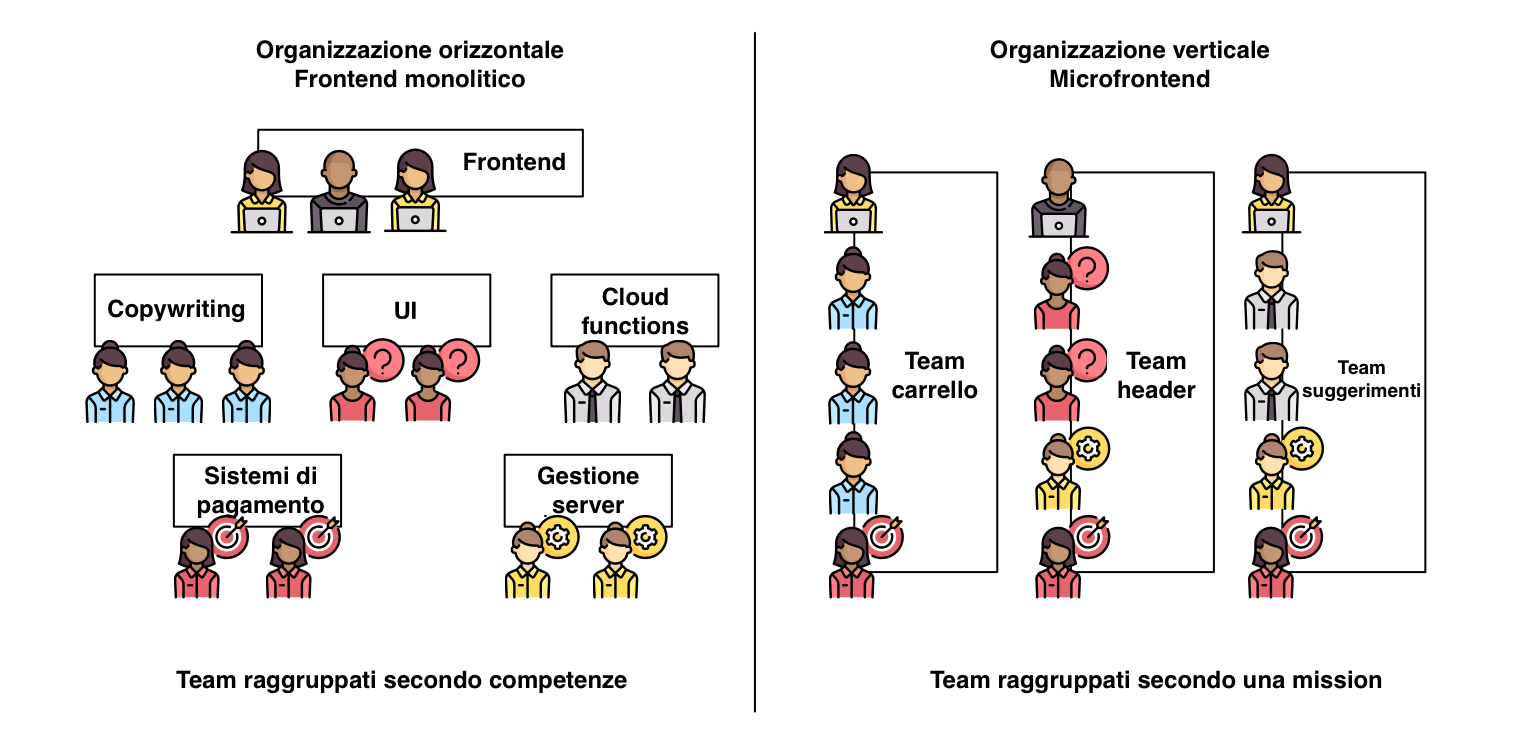
\includegraphics[width=140mm]{img/schema_microfrontend}
  \caption{Differenze di composizione di team tra approccio monolitico e microfrontend}
\end{figure}
L'obiettivo della tecnologia microfrontend è quello di superare l'approccio monolitico, che vede
lo sviluppo di applicazioni web suddiviso in due team: backend e frontend.

Si fa questo vedendo un'applicazione web come un insieme
di elementi, chiamati fragment o microfrontend, molto disaccoppiati tra di loro
e con la più bassa granuralità, ovvero con la funzionalità più minimale possibile.

Ogni microfrontend viene sviluppato da un team, che potrà lavorare con autonomia. 
Essendo i singoli microfrontend autonomi,
questi possono funzionare anche se estratti dalla applicazione web che li contiene,
 e il malfunzionamento di un singolo microfrontend
non compromette la stabilità degli altri.
I team sono autonomi, ma non sono isolati: questi infatti condividono un insieme di dati, che
chiameremo \emph{contratto},
fondamentali per il corretto funzionamento dell'applicazione. A seconda delle tecnologie utilizzate
per realizzare l'architettura microfrontend, il contratto tra i team sarà più o meno complesso.



\subsection{Vantaggi}
\begin{itemize}
    \item \textbf{Ottimizzare lo sviluppo di funzionalità:}
Nell’approccio orizzontale quando si vuole sviluppare una nuova funzionalità è necessario far convergere il 
lavoro di più team. Con microfrontend,
  tutte le persone coinvolte nell’implementazione di una nuova funzionalità sono nello 
  stesso team, rendendo il lavoro più veloce ed efficiente. 
    \item \textbf{Abbandono del frontend monolitico:}
Con microfrontend le applicazioni, incluse il frontend, si dividono in sistemi verticali
 più piccoli. Ogni team controlla la sua piccola parte di frontend e di backend.
    \item \textbf{Adottare diverse tecnologie:}
Strumenti di sviluppo e framework evolvono continuamente. Ogni team deve essere in grado di scegliere
le proprie tecnologie autonomamente. Ci sono alcune grandi aziende
 come Github, che hanno
 impiegato molto tempo per eliminare alcune dipendenze ormai obsolete dal loro codice ( nel caso di Github si trattava di una versione di JQuery).
  Con l’approccio microfrontend questi cambiamenti sono più rapidi e possono essere
   fatti modularmente.


\item \textbf{Indipendenza:}
I progetti di ogni team sono autonomi, ovvero non hanno dipendenze condivise tra di loro.
Questo come già detto precedentemente porta ad una grande autonomia.

L’indipendenza però porta sicuramente a costi aggiuntivi. Si potrebbe pensare che sia
 più semplice quindi di sviluppare un unico progetto, e assegnare parti di questo a team diversi. 
 Il problema sta nel fatto che la comunicazione tra i vari team è costosa e porta molti ritardi.
In alcuni casi quindi è preferibile introdurre ridondanza nel codice dei vari team a favore di più autonomia e velocità di
 implementazione.

\end{itemize}

\subsection{Svantaggi}
\begin{itemize}

\item \textbf{Ridondanza:}
In informatica si è addestrati a ridurre al minimo le ridondanze.
Anche nel caso dello sviluppo frontend ci sono degli episodi nei quali la ridondanza può
 essere molto costosa: come ad esempio quando viene trovato un bug in una libreria e 
 questo viene risolto da un team, il fix dovrà essere comunicato agli altri e questi 
 dovranno provvedere a risolverlo autonomamente. Oppure quando si rende un processo più 
 veloce, anche in questo caso va comunicato agli altri team e questi dovranno apprendere
  la scoperta.
Si adotta quindi un approccio microfrontend quando i costi associati a ridondanze sono 
inferiori agli impatti negativi a uno sviluppo frontend monolitico, che porta a forti 
dipendenze tra team.




\item \textbf{Inconsistenza:}
 Potrebbero essere presenti delle basi di dati, necessarie all'applicazione web, che vengono lette e scritte
 da più microfrontends.
Per garantire la proprietà di indipendenza tra team è necessario replicare il database per tutti i progetti. 
Tutte queste copie devono però essere sincronizzate tra loro regolarmente per mantenere la consistenza e la coerenza dei dati.
Questo introduce dei ritardi, che potrebbero penalizzare l'esperienza utente.

\item \textbf{Eterogeneità:}
Potrebbe essere controverso avere la libertà di utilizzare tecnologie diverse tra i vati team.
 Ovviamente se ogni team usa una diversa tecnologia lo scambio di pareri o di competenze 
 tra team diventa più difficile.
\end{itemize}
\chapter{Collegare i microfrontends}\label{ch:composizione}
Per far convivere i progetti realizzati dai vari team esistono varie metodologie. Questo
 presuppone che i team, nella loro autonomia, debbano comunque scambiarsi un minimo di informazioni e di vincoli
che servono alla corretta integrazione delle app web, chiamiamo questo insieme di dati \emph{contratto tra team}.

\section*{Collegamento tra pagine con links}
La soluzione più semplice è quella del collegamento tra pagine con link URL: in questo modo il contratto consiste negli indirizzi delle pagine,
che i team dovranno scambiarsi tra di loro.
Questa soluzione è quella che rende i team il più autonomi e disaccoppiati possibile, inoltre
si ha grande robustezza, in quanto se un progetto si corrompe, questo non influenza minimamente gli altri,
che possono anche essere detenuti in server diversi.

Lo svantaggio è che in una pagina web è possibile contenere informazioni provenienti da un solo team.

Questa soluzione viene usata quando è richiesta una forte robustezza, oppure quando si deve implementare 
i microfrontends in una app legacy già esistente.


\section*{Composizione tramite iframes}
L' iframe è un elemento HTML che permette di incorporare un'altra pagina HTML all'interno di quella corrente. \cite{mozillaiframe}

Questo elemento può essere usato per comporre fragments provenienti da teams differenti, visualizzandoli su un'unica
pagina web.
Un team si impegnerà a realizzare la pagina ospitante e dovrà far presente agli altri attori lo spazio riservato
ai loro fragments per evitare problemi di visualizzazione, questo dato, oltre che agli indirizzi
URL delle varie pagine, farà parte del contratto tra i team.

Un grande svantaggio dell’uso degli iframes è la loro incompatibilità con i motori di ricerca.
Infatti le informazioni che vediamo nella pagina non sono in unico file HTML, di conseguenza il motore di ricerca non profila le informazioni 
contenute negli iframes.

\subsection*{Composizione con Ajax}
Un modo per superare il problema dei motori di ricerca ai quali sono affetti gli iframes è quello di 
caricare i file HTML con Ajax.

La pagina ospitante, detta \emph{wrapper} ha il compito di caricare nel proprio DOM ( Document Object Model) i fragments dei vari 
team, con l'ausilio di un codice javascript, che utilizza la funzione fetch().

Il problema principale però è che l’Ajax request è asincrona, 
questo porta a dei ritardi nel caricamento completo della pagina.

\subsection*{Utilizzo del Routing Server-side}
Il routing è un elemento fondamentale dell’architettura microfrontend.
L’elemento che stiamo introducendo viene chiamato frontend proxy, cioè un web server che effettua routing,
 che intercetta le richieste con un certo percorso e le instrada al giusto fragment. In questo modo anche se
  i progetti dei vari team risiedono in spazi diversi, l’utente vedrà un URL omogeneo e non si accorgerà delle origini dei fragment.
Il funzionamento consiste in questi passaggi:
\begin{itemize}
    \item Il client apre l’ URL “/foo/bar”. La richiesta raggiunge il frontend proxy
    \item Il frontend proxy confronta il path “/foo/bar/“8 con la propria routing table, con corrispondenza in prossimità della regola i
    \item Il frontend proxy passa la richiesta al fragment associato
    \item Il fragment genera una risposta e la ritorna al frontdend proxy
    \item La risposta arriva infine al client
\end{itemize}


\pagebreak

\section*{Composizione Server-side}
Si suppone di lavorare ad un progetto microfrontend incentrato principalmente su contenuti e informazioni, senza particolari applicativi logici al suo interno.
Un esempio di sito incentrato sulle informazioni( anche detto \emph{content-centric}) è Wikipedia, le sue caratteristiche principali sono:
\begin{enumerate}
    \item Tempi brevi di caricamento delle pagine
    \item Ottimizzazione per motori di ricerca
    \item Assenza di particolari contenuto logici basati sull'interazione con l'utente
\end{enumerate}

Si introduce quindi la \textbf{composizione server-side}, che rispetta le richieste di un sito content-centric come Wikipedia.

La composizione dei fragment viene eseguita da un servizio che risiede nel server web, il client quindi riceve la pagina completa.

Come nel caso degli iframes, i team che producono i fragments devono fornire al team che detiene la pagina ospitante l'URL del loro codice di markup HTML.

Il team della pagina ospitante userà delle direttive 
per richiedere al server di aggiungere il codice di markup degli altri team in un preciso posto della schermata.

Un esempio di servizio di composizione è la funzione \textbf{SSI} (Server-Side Includes) di \textbf{Nginx}:

\subsection*{Server-Side Includes}

Nginx contiene il modulo \emph{ngx-http-ssi-module} che processa i comandi SSI.
 I comandi SSI sono istruzioni
inserite nelle pagine HTML della pagina ospitante. Un'istruzione SSI appare nella seguente sintassi:

   \begin{center}
    \verb|<!--#include virtual="url/da/includere -->|
   \end{center}

Avviene quindi questo:

\begin{enumerate}
    \item Il client effettua la richiesta della pagina
    \item Il webserver accetta la richiesta e verifica la presenza di eventuali direttive SSI
    \item Le direttive trovate vengono sostituite con il codice di markup reperibile all'url dell'attributo "virtual"
    \item Il client riceve la pagina completa
\end{enumerate}

Si noti che le prestazioni di composizione sono nettamente aumentate rispetto alla composizione con iframes, 
in quanto il client riceve la pagina già completa, effettuando un solo handshake HTML, indipendentemente dal numero
di fragment ospitati nella pagina. Inoltre i motori di ricerca possono profilare anche il contenuto dei fragments

\subsubsection*{Modalità di caricamento dei fragments}
Al contrario della soluzione con iframes, lo scorretto caricamento di un fragment può rallentare o addirittura bloccare 
il caricamento dell'intera pagina. Il webserver infatti prima di restituire la pagina aspetta di avere tutti  i suoi componenti.
La proprietà di Nginx chiamata \emph{proxy read timeout} permette di fissare un tempo massimo per il quale il webserver 
può aspettare un fragment.

Nel caso in cui il webserver non riesce a caricare un fragment esiste il comando SSI \textbf{stub}.
Si utilizza la direttiva \emph{block} che sostiuirà il fragment caricato senza successo con del codice HTML di riserva.
Il nuovo \emph{include} contiene il nuovo attributo stub, che ha il riferimento al block corrispondente, dovesse non andare
a buon fine la richiesta.


\verb|<!--# block name="fallback" -->|\linebreak
\verb|<a href="/page"> Link</a>|\linebreak
\verb|<!--# endblock -->|\linebreak
\verb| <!--#include|\linebreak
\verb|virtual="/link/to/page"|\linebreak
\verb| stub="fallback" -->|\linebreak

\linebreak
Quando Nginx deve scaricare più fragments, effettua i caricamenti in parallelo.
Quando l'ultimo fragment viene scaricato,la pagina viene composta e inviata al client.
Il tempo di risposta dell'intera pagina è chiamato \emph{time to first byte} (TTFB) ed è definito 
come il tempo necessario per generare l’HTML della pagina, più il tempo di caricamento del fragment più lento.

E' possibile anche annidare fragments, ma non è consigliato, in quanto si 
interrompe la parallelizzazione dei caricamenti e si rallenta la composizione della pagina.

\subsubsection*{Caricamento differito}
In genere si ottimizza il caricamento della pagina effettuando una composizione server-side per la sua parte principale,
 la cosiddetta \emph{viewport}, le componenti secondarie invece è preferibile comporle lato client, con 
delle chiamate Ajax, utilizzando la metodologia prima descritta. Questa tecnica si chiama caricamento differito, o \textbf{lazy loading}.

\subsubsection*{Alternative a SSI}
Il webserver con SSI, invia la pagina al client solo quando questa è stata completamente composta.
Il servizio di composizione \textbf{ESI} presente nel webserver Vernish invece attua l'\emph{invio parziale},
 ovvero inizia a inviare parti di pagina anche prima che questa venga completamente assemblata.

Esistono altre soluzioni, come quella sviluppata dalla società di fashion e-commerce Zalando, chimata Zalando Tailor.
L'azienda migrò infatti il loro microfrontend dall'approccio monolitico a quello microfrontend, utilizzando una composizione
server-side. Per via dell'entità del sito web, il team Zalando ha avviato il progetto Tailor, che ha poi portato ad un rilascio 
ufficiale con licenza \textbf{TODOlibera}. Tailor consiste in una libreria Node.js, reperibile nel pacchetto NPM \emph{node-tailor}.

Tailor riesce ad avere prestazioni migliori rispetto all'invio parziale, facendo in modo di iniziare a inviare parti di pagina al client,
ancora prima che il server abbia finito di scaricare l'intera pagina.

\pagebreak
\section*{Composizione Client-side}
Ci sono dei siti web che non hanno principalmente uno scopo informativo, ma funzionale, ovvero rispondono all'input dell'utente
e rilasciano un output influenzato da tale input. Questi siti web vengono detti \emph{behavior-centric}, cioè 
incentrati su un comportamento o funzionalità.
Il modo più indicato per chiamarli non è siti web ma web apps, applicazioni web.
Una web app è ad esempio Google Meet, raggiungibile dall'URL https://meet.google.com.
Questo non è un sito che veicola principalmente informazioni, ma bensì offre un servizio all'utente: permette a due o più persone di 
interloquire, tramite scambio di segnali audiovisivi. Per fare in modo di reagire
all input degli utenti, le webapp cambiano il loro codice HTML nel browser, e inoltre permettono 
di cambiare pagina, e quindi anche URL, senza effettuare alcuna richiesta al webserver.
Sono disponibili agli sviluppatori numerosi framework per realizzare webapps, come React.js, Angular e Vue.js.
Seguendo un approccio monolitico dovremmo scegliere uno di questi framework ed essere costretti a farlo utilizzare
a tutti i team che lavorano al progetto. Al contrario, con l'approccio microfrontend, si da libertà ad ogni team
di scegliere autonomamente la soluzione migliore e di mantenerla aggiornata.
Grazie agli \textbf{web components}, i team possono realizzare dei fragments con qualsiasi tecnologia a loro disposizione e 
farli operare con il resto della pagina.



\subsection*{Web Components}
Gli web components consentono di creare nuovi elementi HTML personalizzati ( Custom Elements), riutilizzabili e incapsulati
da utilizzare in siti e web app \cite{webcomponents}.

Custom Elements è un insieme di API Javascript che consentono di definire elementi HTML personalizzati, che includono istruzioni CSS e JS.
Ogni custom element è dichiarato nell' oggetto \emph{CustomElementRegistry}.
\linebreak

All'interno di un web component può essere incapsulato elementi di stile e componenti logiche, senza influenzare
la parte restante del DOM (Document Object Model), questo grazie alla \emph{shadow DOM}:
\subsubsection*{Shadow DOM}
Sappiamo che il DOM (Document Object Model) è un albero di oggetti creato alla fine del caricamento di ogni pagina web, che 
permette di accedere dinamicamente e aggiornare il contenuto, la struttura e lo stile di un documento.\cite{dom}
Possiamo annettere alla struttura del DOM, un numero arbitrario di \emph{shadow trees}, 
o alberi ombra, questi con i loro elementi e il proprio design hanno una radice, detta  \emph{shadow root}.
La shadow root è sempre annessa ad un \emph{shadow host} che risiede nel DOM o in un altro shadow tree.

Grazie alla Shadow DOM è possibile gestire singoli elementi di un progetto web in modo indipendente rispetto al resto del sito.
Dentro la shadow DOM è possibile gestire contenuti in maniera del tutto indipendente rispetto alle istruzioni di design o dalle strutture
valide globalmente nel resto del progetto.

Questo aumenta la robustezza del microfrontend, garantendo isolamento.
\linebreak
\linebreak
Un altro elemento importante che sta alla base dei web components è il concetto di \textbf{template HTML}: 
un modo per creare codice HTML non ancora visualizzato sulla pagina, che può essere istanziato una o più volte 
durante il runtime grazie a codice javascript.



\subsection*{Comunicazione tra fragments}
I fragment possono aver bisogno di ricevere dalla pagina 
ospitante delle informazioni di contesto, come ad esempio la lingua, 
la regione geografica, o il nome dell'utente recuperata da un database.
Gli attributi dei custom element possono fungere da mezzo di comunicazione per inviare
informazioni dalla pagina al fragment.
I custom elements, con i quali sono implementati gli web components, forniscono agli sviluppatori 
una serie di metodi che interessano momenti del loro ciclo di vita:
\begin{itemize}
    \item \textbf{connectedCallback}: invocato quando il custom element viene inserito nel DOM della pagina 
    \item \textbf{disconnectedCallback}: invocato quando il custom element viene rimosso dal DOM
    \item \textbf{adoptedCallback}: invocato quando l'elemento viene spostato da un documento ad un altro
    \item \textbf{attributeChangedCallback}: invocato quando un qualsiasi attributo del documento cambia
\end{itemize}

Si può quindi utilizzare il metodo \emph{attributeChangedCallback} per far reagire il fragment in risposta ad un
attributo cambiato.

\linebreak

Per quanto riguarda la comunicazione da un fragment alla pagina, è possibile utilizzare 
l'API nativa \textbf{CustomEvents}, disponibile in tutti i moderni browsers.
Permette di emettere eventi personalizzati allo stesso modo di come funzionano gli eventi standard \emph{click} o \emph{change}.

Per far si che il colloquio vada a buon fine, il team che gestisce il fragment deve comunicare a quello che gestisce la pagina
il nome dell'evento.

\pagebreak

Analizziamo adesso le diverse strategie per far comunicare due fragment ospitati sulla stessa pagina:

\begin{itemize}
    \item \textbf{Comunicazione diretta}: consiste nel chiamare direttamente il metodo del fragment
    interessato, secondo il principio che qualsiasi fragment ha accesso all'intero DOM della pagina.
    Questo metodo è altamente sconsigliato, perchè introduce un \textbf{forte accoppiamento}
    \item \textbf{comunicazione tramite pagina ospitante}: si usa la pagina ospitante come tramite del messaggio,
    utilizzando le tecniche prima viste, si emette un evento dal fragment A, si riceve nella pagina, e si inoltra ad un attributo 
    del fragment B.
    \item \textbf{Broadcast Channel API}: la Broadcast channel API permette la comunicazione 
    tra elementi del browser della stessa \emph{origin}, ovvero con hostname, e porta uguali. 
    Si basa sul meccanismo publish/subscribe.
    Vengono instaurati dei canali nei quali vengono pubblicati messaggi (\emph{publish}), 
    che riceveranno solo i fragment che si sottoscrivono a tale canale(\emph{subscribe}).
    Questa soluzione riduce al minimo l'accoppiamento tra i vari fragments.
    Broadcast channel API verrà approfondito successivamente.
\end{itemize}

E' importante che le comunicazioni tra i fragemnt siano minime e che interessino dati semplici, in quanto
un eccessivo accoppiamento tra due oggetti può significare un inesatto confine tra due team.


\subsection*{Application Shell}


\subsubsection*{Routing a due livelli}




\pagebreak
\section*{Universal Rendering}
\chapter{Conclusioni}\label{ch:conclusioni}
Come lo sono i microservizi per il lato backend, i microfrontend sono un efficace soluzione per dividere i compiti tra team omogenei
e realizzare un progetto web modulare e reattivo ai cambiamenti. Ogni team produce delle applicazioni indipendenti, 
che possono essere estratte dal contesto e riproposte in altri progetti che richiedono funzionalità analoghe.
Numerose aziende hanno migrato verso questa tecnologia, una di queste è la tedesca Zalando, leader nel settore e-commerce, che con
il progetto Mosaic ha rilasciato pubblicamente una raccolta di servizi e librerie per aiutare proprietari di grandi siti web a migrare 
dall'approccio monolitico, contribuendo la diffusione di tale pratica rendendola più accessibile \cite{mosaic}, non si deve trascurare il fatto che 
realizzare un progetto web con questa architettura è molto più complesso di farlo con l'approccio monolitico, o almeno inizialmente.

Una parola ricorrente in questo elaborato è \textbf{composizione}: ovvero il far convivere nella solita finestra del browser
più fragments provenienti da team diversi. La composizione può essere effettuata prima di far arrivare la pagina al client, oppure
dopo, delegando l'operazione al browser.

Molto spesso si è parlato di \textbf{autonomia}, che non vuol dire isolamento: i team lavorano per lo più internamente, ma 
a seconda delle tecnologie utilizzate, devono presentare agli altri un \emph{contratto}, delle informazioni che devono essere condivise
per mettere in fase l'intero progetto. Queste informazioni però devono restare minime, 
perche quanto più il contratto è pieno di "clausole" da rispettare, tanto più il progetto si complica.

La piattaforma Leonardo X2030 è l'esempio perfetto per la messa in opera di un'architettura microfrontend:
contiene molti strumenti, ha un'interfaccia modulare personalizzabile al massimo, è aggioranta continuamente
per essere compatibile con le nuove tecnologie, come rilievi con droni o gestione di big data sfruttando l'intelligenza artificiale.
Tutte queste funzionalità eterogenee devono comunicare tra di loro, e devono essere racchiuse in un interfaccia che le
renda utilizzabili contemporaneamente al personale di diversi enti.


\addcontentsline{toc}{chapter}{Bibliografia}
\bibliographystyle{plain}
\bibliography{files/biblio}
\bibliographystyle{unsrt}
%\bibliography{sp,xml}

\end{document} 